\apendice{Especificación de Requisitos}

\section{Introducción}

\section{Objetivos generales}

\section{Catalogo de requisitos}
En esta sección se presentan los requisitos funcionales y los no funcionales
\subsection{Requisitos funcionales}\label{requisitos-funcionales}
\begin{itemize}
\tightlist
\item
\textbf{RF-1 Confidencialidad del sistema:} solamente usuarios permitidos podrán acceder al sistema.
	\begin{itemize}
		\tightlist
		\item
		\textbf{RF-1.1 Identificación de usuario:} los usuarios se identificarán con un \textit{nickname} y una contraseña 
		\item
		\textbf{RF-1.2 Rol de administración:} existirá un usuario especial que podrá administrar el sistema completamente sin restricciones.
		\item 
		\textbf{RF-1.3 Visualización de una cama:} los usuarios validados deben poder observar los datos en tiempo real de las camas disponibles. 
		\item
		\textbf{RF-1.4 Restricción de acceso:} los usuarios solamente podrán tener acceso a los datos de las camas permitidas. 
		\item
		\textbf{RF-1.5 Acceso completo al administrador:} el administrador debe poder acceder a todas las camas existentes. 
	\end{itemize}	
\item
\textbf{RF-2 Gestión de las camas:} el administrador ha de gestionar las camas pudiendo añadir, modificar y borrar.
	\begin{itemize}
		\tightlist
		\item
		\textbf{RF-2.1 Añadir cama:} el administrador ha de poder añadir una nueva cama al sistema.
		\item
		\textbf{RF-2.2 Modificar cama:} el administrador ha de poder modificar los datos una cama existente.
		\item
		\textbf{RF-2.3 Borrar cama:} el administrador ha de poder borrar una cama del sistema.
		\item
		\textbf{RF-2.4 Asignar camas a usuarios:} el administrador se encarga de decidir que usuario puede acceder a que cama.
	\end{itemize}
\item
\textbf{RF-3 Gestión de los usuarios:} el administrador ha de gestionar los usuarios pudiendo añadir, modificar y borrar.
	\begin{itemize}
		\tightlist
		\item
		\textbf{RF-3.1 Añadir usuario:} el administrador ha de poder añadir un nuevo usuario al sistema.
		\item
		\textbf{RF-3.2 Modificar usuario:} el administrador ha de poder modificar los datos un usuario existente.
		\item
		\textbf{RF-3.3 Borrar usuario:} el administrador ha de poder borrar un usuario del sistema.
	\end{itemize}
\item 
\textbf{RF-4 Visualización de los datos:} los usuarios han de poder ver de las camas disponibles el estado actual del paciente, sus constantes vitales y las presiones.
\end{itemize}	
\subsection{Requisitos no funcionales}\label{requisitos-no-funcionales}
\begin{itemize}
\tightlist
\item
\textbf{RNF-1 Usabilidad:} la aplicación debe cumplir estándares de usabilidad teniendo una curva de aprendizaje baja y un uso de metáforas adecuado.
\item 
\textbf{RNF-2 Disponibilidad:} las camas existentes han de ser siempre accesibles por sus usuarios asociados y dar una información correcta de su estado
\item 
\textbf{RNF-3 Confidencialidad:} los datos de las camas, al ser en parte constantes vitales de pacientes, solamente han de ser accesibles por los usuarios permitidos.
\item
\textbf{RNF-4 Escalabilidad:} el sistema debe ser escalable para adaptarse mejor a un incremento de carga del sistema.
\item 
\textbf{RNF-5 Seguridad:} los usuarios deben poder identificarse sólidamente con el sistema sin que sus datos o sus credenciales (\textit{tokens}) sean accesibles por terceros, incluso el administrador.
\item
\textbf{RNF-6 Exstensibilidad:} la API del sistema debe ser fácilmente extensible a nuevas funcionalidades incorporando de manera eficaz soporte a nuevas peticiones.
\item
\textbf{RNF-7 Persistencia:} los servicios de procesamiento de las camas activas deben mantenerse funcionando aunque no existan clientes activos para evitar retrasos muy altos ante nuevas conexiones.
\item
\textbf{RNF-8 Fiabilidad:} los datos de la aplicación son correctos y actuales además de garantizar una predicción óptima del estado del paciente.
\end{itemize}

\section{Especificación de requisitos}\label{casos-uso}

Los requisitos funcionales generan un conjunto de casos de uso que serán la base del desarrollo de la aplicación. La especificación de los mismos se encuentran entre la tabla~\ref{tabla:tablaCU1} y la tabla~\ref{tabla:tablaCU43}. La representación gráfica se puede ver en los diagramas de las figuras~\ref{fig:cu-1} y \ref{fig:cu-2}. Existen dos actores, el \textbf{administrador} que se encarga de toda la labor de gestión tanto de usuarios como de camas y el \textbf{usuario} que únicamente puede gestionarse a si mismo y ver los datos de las camas que tenga permitidas.

\begin{figure}[h]
	\centering
	\begin{subfigure}[b]{0.75\textwidth}
		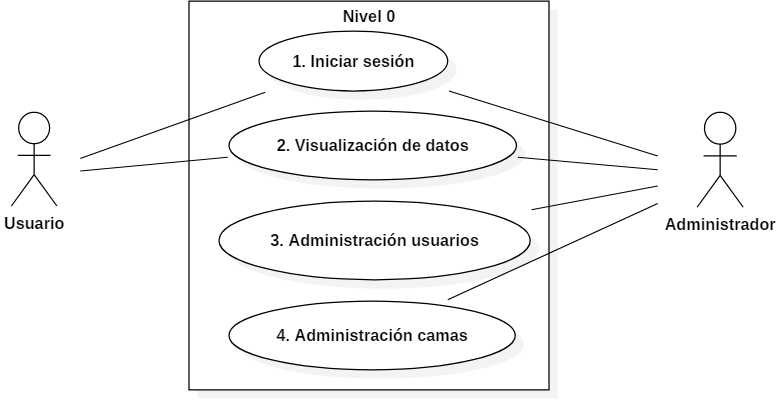
\includegraphics[width=\textwidth]{cu-lv1}
		\caption{Diagrama casos de uso - Nivel 0}
	\end{subfigure}
	\begin{subfigure}[b]{0.75\textwidth}
		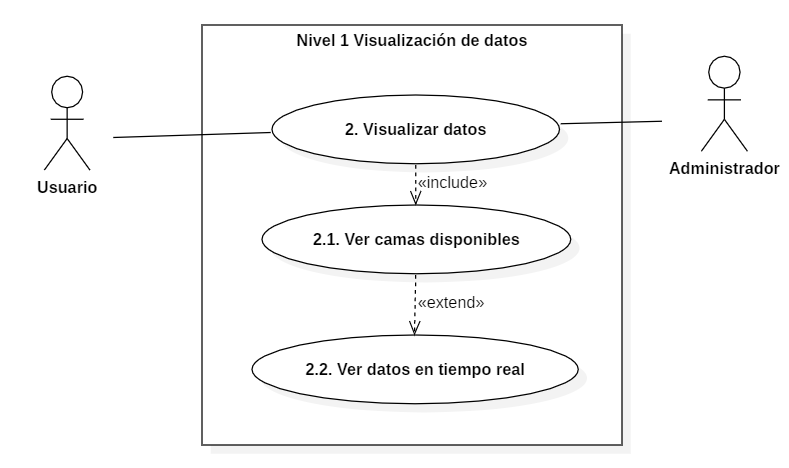
\includegraphics[width=\textwidth]{cu-lv11}
		\caption{Diagrama CU-2 - Nivel 1}
	\end{subfigure}
	\caption{Diagramas de casos de uso}
	\label{fig:cu-1}
\end{figure}

\begin{figure}[h]
	\centering
	\begin{subfigure}[b]{0.75\textwidth}
		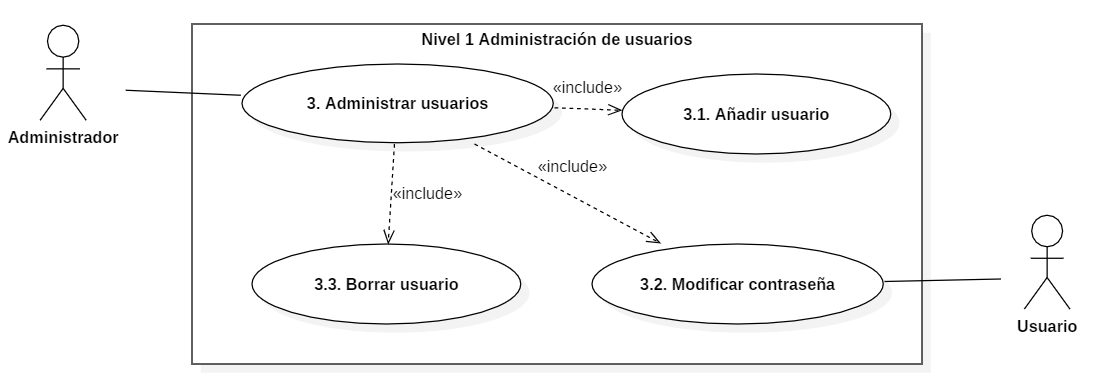
\includegraphics[width=\textwidth]{cu-lv12}
		\caption{Diagrama CU-3 - Nivel 1}
	\end{subfigure}
	\begin{subfigure}[b]{0.75\textwidth}
		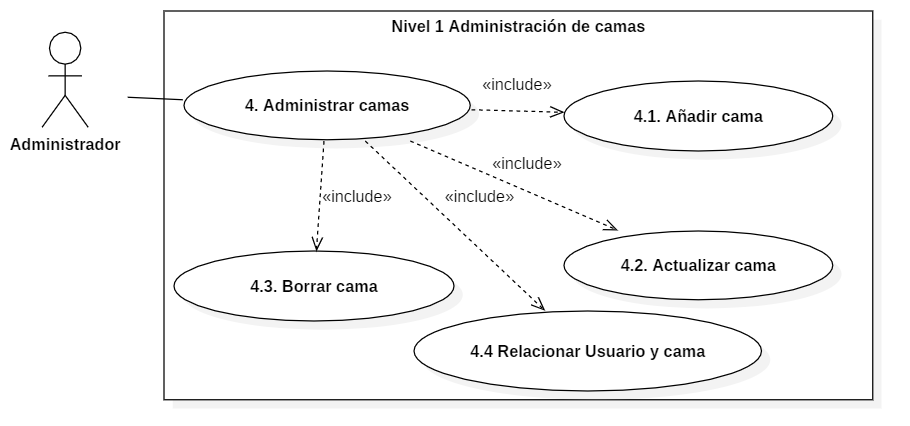
\includegraphics[width=\textwidth]{cu-lv13}
		\caption{Diagrama CU-4 - Nivel 1}
	\end{subfigure}
	\caption{Diagramas de casos de uso}
	\label{fig:cu-2}
\end{figure}

\tablaSmallSinColores{Caso de uso 1: Loguear }{p{3cm} p{.75cm} p{9.5cm}}{tablaCU1}{
	\multicolumn{3}{p{10.25cm}}{CU-1: Loguear} \\
}
{
	Descripción                            & \multicolumn{2}{p{10.25cm}}{El usuario se identifica en el sistema} \\\hubu
	Precondiciones                         & \multicolumn{2}{p{10.25cm}}{No existe una sesión activa válida} \\\hubu
	Requisitos                         	   & \multicolumn{2}{p{10.25cm}}{RF-1, RF-1.1} \\\hubu
	Usuario                         	   & \multicolumn{2}{p{10.25cm}}{Anónimo} \\\hubu
	\multirow{3}{3.5cm}{Secuencia normal}  & Paso & Acción \\\cline{2-3}
	& 1    & El cliente envía sus credenciales al servidor \\\cline{2-3}
	& 2    & El servidor acepta las credenciales devolviendo el token de sesión \\\cline{2-3}
	Postcondiciones                        & \multicolumn{2}{p{10.25cm}}{El usuario tiene una sesión activa válida} \\\hubu
	\multirow{2}{3.5cm}{Excepciones}       & Paso & Acción \\\cline{2-3}
	& 2    & Si las credenciales son incorrectas el servidor responde con error \\\hubu
	Frecuencia                             & Alta \\\hubu
	Importancia                            & Crítico \\\hubu
	Comentarios                            & \multicolumn{2}{p{10.25cm}}{Es siempre lo primero que aparecerá} \\
}

\tablaSmallSinColores{Caso de uso 2: Visualizar de datos }{p{3cm} p{.75cm} p{9.5cm}}{tablaCU2}{
	\multicolumn{3}{p{10.25cm}}{CU-2: Visualizar de datos} \\
}
{
	Descripción                            & \multicolumn{2}{p{10.25cm}}{Ver lista de las camas disponibles} \\\hubu
	Precondiciones                         & \multicolumn{2}{p{10.25cm}}{Sesión activa válida} \\\hubu
	Requisitos                         	   & \multicolumn{2}{p{10.25cm}}{RF-1.3, RF-1.4} \\\hubu
	Usuario                         	   & \multicolumn{2}{p{10.25cm}}{Administrador y Usuario} \\\hubu
	\multirow{3}{3.5cm}{Secuencia normal}  & Paso & Acción \\\cline{2-3}
	& 1    & El cliente solicita ver las camas disponibles \\\cline{2-3}
	Postcondiciones                        & \multicolumn{2}{p{10.25cm}}{El cliente está en la pantalla de camas disponibles} \\\hubu
	Frecuencia                             & Alta \\\hubu
	Importancia                            & Alta \\
}

\tablaSmallSinColores{Caso de uso 2.1: Elegir cama }{p{3cm} p{.75cm} p{9.5cm}}{tablaCU21}{
	\multicolumn{3}{p{10.25cm}}{CU-2.1: Elegir cama} \\
}
{
	Descripción                            & \multicolumn{2}{p{10.25cm}}{Elegir cama} \\\hubu
	Precondiciones                         & \multicolumn{2}{p{10.25cm}}{Sesión activa válida} \\\hubu
	Requisitos                         	   & \multicolumn{2}{p{10.25cm}}{RF-1.3, RF-1.4, RF-4} \\\hubu
	Usuario                         	   & \multicolumn{2}{p{10.25cm}}{Logueado} \\\hubu
	\multirow{3}{3.5cm}{Secuencia normal}  & Paso & Acción \\\cline{2-3}
	& 1    & El cliente solicita ver las camas disponibles \\\cline{2-3}
	& 2    & El servidor abre conexiones paralelas para actualizar en tiempo real el estado de las camas \\\cline{2-3}
	& 3    & El cliente decide que cama ver \\\cline{2-3}
	Postcondiciones                        & \multicolumn{2}{p{10.25cm}}{El cliente entra en la ventana de los datos en tiempo real} \\\hubu
	Frecuencia                             & Alta \\\hubu
	Importancia                            & Alta \\
}

\tablaSmallSinColores{Caso de uso 2.2: Ver datos en tiempo real }{p{3cm} p{.75cm} p{9.5cm}}{tablaCU22}{
	\multicolumn{3}{p{10.25cm}}{CU-2.2: Ver datos en tiempo real} \\
}
{
	Descripción                            & \multicolumn{2}{p{10.25cm}}{Ver datos en tiempo real} \\\hubu
	Precondiciones                         & \multicolumn{2}{p{10.25cm}}{Sesión activa válida y cama existente y accesible} \\\hubu
	Requisitos                         	   & \multicolumn{2}{p{10.25cm}}{RF-1.3, RF-1.4, RF-4} \\\hubu
	Usuario                         	   & \multicolumn{2}{p{10.25cm}}{Administrador y usuario} \\\hubu
	\multirow{3}{3.5cm}{Secuencia normal}  & Paso & Acción \\\cline{2-3}
	& 1    & El cliente solicita una nueva conexión \\\cline{2-3}
	& 2    & El servidor provee una conexión en tiempo real con los datos \\\cline{2-3}
	Postcondiciones                        & \multicolumn{2}{p{10.25cm}}{El usuario tiene una conexión paralela abierta con los datos en tiempo real} \\\hubu
	\multirow{2}{3.5cm}{Excepciones}       & Paso & Acción \\\cline{2-3}
	& 2    & Si un paquete faltase o la señal fuera débil se alertaría al usuario \\\cline{2-3}
	Frecuencia                             & Alta \\\hubu
	Importancia                            & Máxima \\}

\tablaSmallSinColores{Caso de uso 3: Administrar de usuarios }{p{3cm} p{.75cm} p{9.5cm}}{tablaCU3}{
	\multicolumn{3}{p{10.25cm}}{CU-3: Administrar de usuarios} \\
}
{
	Descripción                            & \multicolumn{2}{p{10.25cm}}{Administración de usuario: alta, baja y modificación} \\\hubu
	Precondiciones                         & \multicolumn{2}{p{10.25cm}}{Sesión de administrador válida} \\\hubu
	Requisitos                         	   & \multicolumn{2}{p{10.25cm}}{RF-3} \\\hubu
	Usuario                         	   & \multicolumn{2}{p{10.25cm}}{Administrador} \\\hubu
	\multirow{3}{3.5cm}{Secuencia normal}  & Paso & Acción \\\cline{2-3}
	& 1    & El administrador entra en el menú de administración de usuarios \\\cline{2-3}
	Postcondiciones                        & \multicolumn{2}{p{10.25cm}}{El administrador está en el menú de administración de usuarios} \\\hubu
	Frecuencia                             & Baja \\\hubu
	Importancia                            & Alta \\
}

\tablaSmallSinColores{Caso de uso 3.1: Añadir usuarios }{p{3cm} p{.75cm} p{9.5cm}}{tablaCU31}{
	\multicolumn{3}{p{10.25cm}}{CU-3.1: Añadir usuarios} \\
}
{
	Descripción                            & \multicolumn{2}{p{10.25cm}}{Añadir usuarios} \\\hubu
	Precondiciones                         & \multicolumn{2}{p{10.25cm}}{Sesión de administración activa} \\\hubu
	Requisitos                         	   & \multicolumn{2}{p{10.25cm}}{RF-3.1} \\\hubu
	Usuario                         	   & \multicolumn{2}{p{10.25cm}}{Administrador} \\\hubu
	\multirow{3}{3.5cm}{Secuencia normal}  & Paso & Acción \\\cline{2-3}
	& 1    & El administrador elige añadir un nuevo usuario \\\cline{2-3}
	& 2    & Se introduce un nombre de usuario para identificarlo \\\cline{2-3}
	& 3    & Se introduce una contraseña dos veces \\\cline{2-3}
	& 4    & Se almacenan los datos \\\cline{2-3}
	Postcondiciones                        & \multicolumn{2}{p{10.25cm}}{Existe un nuevo usuario en el sistema} \\\hubu
	\multirow{2}{3.5cm}{Excepciones}       & Paso & Acción \\\cline{2-3}
	& 2    & Si el nickname existiese \\\cline{2-3}
	& 3    & La contraseña añadida no coincide en las dos ocasiones \\\cline{2-3}
	Frecuencia                             & Baja \\\hubu
	Importancia                            & Alta \\
}

\tablaSmallSinColores{Caso de uso 3.2: Modificar contraseña }{p{3cm} p{.75cm} p{9.5cm}}{tablaCU32}{
	\multicolumn{3}{p{10.25cm}}{CU-3.2: Modificar contraseña} \\
}
{
	Descripción                            & \multicolumn{2}{p{10.25cm}}{Cambiar la contraseña de un usuario} \\\hubu
	Precondiciones                         & \multicolumn{2}{p{10.25cm}}{Sesión activa válida, usuario existente} \\\hubu
	Requisitos                         	   & \multicolumn{2}{p{10.25cm}}{RF-3.2} \\\hubu
	Usuario                         	   & \multicolumn{2}{p{10.25cm}}{Administrador y Usuario} \\\hubu
	\multirow{3}{3.5cm}{Secuencia normal}  & Paso & Acción \\\cline{2-3}
	& 1    & Si es usuario normal ir a 3 \\\cline{2-3}
	& 2    & Si es administrador elegir a qué usuario cambiar la contraseña \\\cline{2-3}
	& 3    & Se introduce una contraseña nueva dos veces \\\cline{2-3}
	& 4    & Se actualizan los datos \\\cline{2-3}
	Postcondiciones                        & \multicolumn{2}{p{10.25cm}}{La contraseña ha cambiado} \\\hubu
	\multirow{2}{3.5cm}{Excepciones}       & Paso & Acción \\\cline{2-3}
	& 3    & La contraseña añadida no coincide en las dos ocasiones \\\cline{2-3}
	Frecuencia                             & Baja \\\hubu
	Importancia                            & Alta \\
}

\tablaSmallSinColores{Caso de uso 3.3: Borrar usuario }{p{3cm} p{.75cm} p{9.5cm}}{tablaCU33}{
	\multicolumn{3}{p{10.25cm}}{CU-3.3: Borrar usuario} \\
}
{
	Descripción                            & \multicolumn{2}{p{10.25cm}}{Elimina un usuario de la base de datos} \\\hubu
	Precondiciones                         & \multicolumn{2}{p{10.25cm}}{Sesión de administración válida, usuario existente} \\\hubu
	Requisitos                         	   & \multicolumn{2}{p{10.25cm}}{RF-3.3} \\\hubu
	Usuario                         	   & \multicolumn{2}{p{10.25cm}}{Administrador} \\\hubu
	\multirow{3}{3.5cm}{Secuencia normal}  & Paso & Acción \\\cline{2-3}
	& 1    & Elegir a que usuario (no administrador) eliminar \\\cline{2-3}
	& 2    & Eliminar usuario y todos los datos vinculados \\\cline{2-3}
	Postcondiciones                        & \multicolumn{2}{p{10.25cm}}{El usuario ha sido eliminado} \\\hubu
	Frecuencia                             & Baja \\\hubu
	Importancia                            & Media \\
}

\tablaSmallSinColores{Caso de uso 4: Administrar de camas }{p{3cm} p{.75cm} p{9.5cm}}{tablaCU4}{
	\multicolumn{3}{p{10.25cm}}{CU-4: Administrar de camas} \\
}
{
	Descripción                            & \multicolumn{2}{p{10.25cm}}{Administración de camas: alta, baja, modificación y asignación a usuarios} \\\hubu
	Precondiciones                         & \multicolumn{2}{p{10.25cm}}{Sesión de administración válida} \\\hubu
	Requisitos                         	   & \multicolumn{2}{p{10.25cm}}{RF-2} \\\hubu
	Usuario                         	   & \multicolumn{2}{p{10.25cm}}{Administrador} \\\hubu
	\multirow{3}{3.5cm}{Secuencia normal}  & Paso & Acción \\\cline{2-3}
	& 1    & El administrador entra en el menú de administración de camas \\\cline{2-3}
	Postcondiciones                        & \multicolumn{2}{p{10.25cm}}{El administrador está en el menú de administración de camas} \\\hubu
	Frecuencia                             & Baja \\\hubu
	Importancia                            & Media \\
}

\tablaSmallSinColores{Caso de uso 4.1: Añadir cama }{p{3cm} p{.75cm} p{9.5cm}}{tablaCU41}{
	\multicolumn{3}{p{10.25cm}}{CU-4.1: Añadir cama} \\
}
{
	Descripción                            & \multicolumn{2}{p{10.25cm}}{Añadir cama} \\\hubu
	Precondiciones                         & \multicolumn{2}{p{10.25cm}}{Sesión de administración válida} \\\hubu
	Requisitos                         	   & \multicolumn{2}{p{10.25cm}}{RF-2.1} \\\hubu
	Usuario                         	   & \multicolumn{2}{p{10.25cm}}{Administrador} \\\hubu
	\multirow{3}{3.5cm}{Secuencia normal}  & Paso & Acción \\\cline{2-3}
	& 1    & El administrador elige añadir una nueva cama \\\cline{2-3}
	& 2    & Se introduce el grupo multicast de la cama (IP y Puerto) \\\cline{2-3}
	& 3    & Se introduce el nombre identificador\\\cline{2-3}
	& 4    & Se almacenan los datos \\\cline{2-3}
	Postcondiciones                        & \multicolumn{2}{p{10.25cm}}{Existe una nueva cama en el sistema} \\\hubu
	\multirow{2}{3.5cm}{Excepciones}       & Paso & Acción \\\cline{2-3}
	& 2    & El grupo multicast pertenece a otra cama \\\cline{2-3}
	& 3    & El nombre identificativo existe para otra cama \\\cline{2-3}
	Frecuencia                             & Media \\\hubu
	Importancia                            & Crítica \\\hubu
	Comentarios                            & \multicolumn{2}{p{10.25cm}}{El grupo multicast se configura en la cama y el administrador solamente debe conocerlo, no configurar la cama física} \\
}

\tablaSmallSinColores{Caso de uso 4.2: Modificar cama }{p{3cm} p{.75cm} p{9.5cm}}{tablaCU42}{
	\multicolumn{3}{p{10.25cm}}{CU-2.2: Modificar cama} \\
}
{
	Descripción                            & \multicolumn{2}{p{10.25cm}}{Modificar los datos de la cama} \\\hubu
	Precondiciones                         & \multicolumn{2}{p{10.25cm}}{Sesión de administración valida, cama existente} \\\hubu
	Requisitos                         	   & \multicolumn{2}{p{10.25cm}}{RF-2.2} \\\hubu
	Usuario                         	   & \multicolumn{2}{p{10.25cm}}{Administrador} \\\hubu
	\multirow{3}{3.5cm}{Secuencia normal}  & Paso & Acción \\\cline{2-3}
	& 1    & Se elige que cama modificar \\\cline{2-3}
	& 2    & Se actualizan los datos a conveniencia del administrador según CU-4.1\\\cline{2-3}
	& 4    & Se actualizan los datos \\\cline{2-3}
	Postcondiciones                        & \multicolumn{2}{p{10.25cm}}{Los datos de la cama se modifican} \\\hubu
	\multirow{2}{3.5cm}{Excepciones}       & Paso & Acción \\\cline{2-3}
	& 2    & Mismas excepciones que en CU-4.1 \\\cline{2-3}
	Frecuencia                             & Baja \\\hubu
	Importancia                            & Alta \\
}

\tablaSmallSinColores{Caso de uso 4.3: Borrar cama }{p{3cm} p{.75cm} p{9.5cm}}{tablaCU43}{
	\multicolumn{3}{p{10.25cm}}{CU-4.3: Borrar cama} \\
}
{
	Descripción                            & \multicolumn{2}{p{10.25cm}}{Elimina una cama de la base de datos} \\\hubu
	Precondiciones                         & \multicolumn{2}{p{10.25cm}}{Sesión de administrador válida, cama existente} \\\hubu
	Requisitos                         	   & \multicolumn{2}{p{10.25cm}}{RF-2.3} \\\hubu
	Usuario                         	   & \multicolumn{2}{p{10.25cm}}{Administrador} \\\hubu
	\multirow{3}{3.5cm}{Secuencia normal}  & Paso & Acción \\\cline{2-3}
	& 1    & Elegir a que cama eliminar \\\cline{2-3}
	& 2    & Eliminar cama y todos los datos vinculados \\\cline{2-3}
	Postcondiciones                        & \multicolumn{2}{p{10.25cm}}{La cama ya no está en la base de datos} \\\hubu
	Frecuencia                             & Baja \\\hubu
	Importancia                            & Media \\
}

\tablaSmallSinColores{Caso de uso 4.4: Asignar cama a usuario }{p{3cm} p{.75cm} p{9.5cm}}{tablaCU43}{
	\multicolumn{3}{p{10.25cm}}{CU-4.4: Asignar cama a usuario} \\
}
{
	Descripción                            & \multicolumn{2}{p{10.25cm}}{Permite a un usuario ver los datos de una cama o quitar ese permiso} \\\hubu
	Precondiciones                         & \multicolumn{2}{p{10.25cm}}{Sesión de administración válida, cama y usuario existentes} \\\hubu
	Requisitos                         	   & \multicolumn{2}{p{10.25cm}}{RF-2.4} \\\hubu
	Usuario                         	   & \multicolumn{2}{p{10.25cm}}{Administrador} \\\hubu
	\multirow{3}{3.5cm}{Secuencia normal}  & Paso & Acción \\\cline{2-3}
	& 1    & Elegir cama \\\cline{2-3}
	& 2    & Elegir usuario \\\cline{2-3}
	& 3    & Si la relación existe se puede eliminar el permiso \\\cline{2-3}
	& 3    & Si la relación no existe se puede crear el permiso \\\cline{2-3}
	Postcondiciones                        & \multicolumn{2}{p{10.25cm}}{El usuario tiene acceso a la cama, o pierde el mismo} \\\hubu
	Frecuencia                             & Media \\\hubu
	Importancia                            & Crítica \\
}